% ============================================================
%  SHIKSHA SETU -- WADHWANI AI HACKATHON PRESENTATION
%  Slides 1-13  |  Compile: pdflatex (x2)
%  No tcolorbox. Uses only core Beamer + tikz + xcolor.
% ============================================================
\documentclass[aspectratio=169,10pt]{beamer}

\usepackage[T1]{fontenc}
\usepackage[utf8]{inputenc}
\usepackage{lmodern}
\usepackage{xcolor}
\usepackage{tikz}
\usepackage{graphicx}
\usepackage{booktabs}
\usepackage{array}
\usepackage{tabularx}
\usepackage{amsmath}
\usepackage{textcomp}
\usetikzlibrary{positioning, shapes.geometric, arrows.meta, calc, backgrounds}

% ── Colours ──────────────────────────────────────────────────
\definecolor{navybg}{HTML}{0F172A}
\definecolor{teal}{HTML}{0D9488}
\definecolor{teallt}{HTML}{14B8A6}
\definecolor{orng}{HTML}{F97316}
\definecolor{card}{HTML}{1E293B}
\definecolor{cardbdr}{HTML}{334155}
\definecolor{txt}{HTML}{F1F5F9}
\definecolor{txtsec}{HTML}{94A3B8}
\definecolor{red}{HTML}{F43F5E}
\definecolor{green}{HTML}{10B981}
\definecolor{purple}{HTML}{8B5CF6}
\definecolor{yellow}{HTML}{F59E0B}

% ── Theme ────────────────────────────────────────────────────
\usetheme{default}
\setbeamercolor{background canvas}{bg=navybg}
\setbeamercolor{normal text}{fg=txt}
\setbeamercolor{frametitle}{fg=teallt, bg=navybg}
\setbeamercolor{footline}{fg=txtsec, bg=navybg}
\setbeamerfont{frametitle}{size=\large,series=\bfseries}
\setbeamertemplate{navigation symbols}{}
\setbeamertemplate{itemize item}{\textcolor{teal}{\textbullet}}
\setbeamertemplate{itemize subitem}{\textcolor{orng}{--}}
\setbeamersize{text margin left=8pt, text margin right=8pt}

% ── Frametitle ───────────────────────────────────────────────
\setbeamertemplate{frametitle}{%
  \vspace{0.25em}%
  \textcolor{teallt}{\textbf{\insertframetitle}}%
  \ifx\insertframesubtitle\empty\else
    \quad\textcolor{txtsec}{\small\insertframesubtitle}%
  \fi\\[-2pt]
  \textcolor{teal}{\rule{\textwidth}{1pt}}%
  \vspace{0.15em}
}

% ── Footer ───────────────────────────────────────────────────
\setbeamertemplate{footline}{%
  \vspace{2pt}
  \hspace{8pt}\textcolor{txtsec}{\footnotesize
    \textbf{\textcolor{teal}{Shiksha Setu}} \;|\; Wadhwani AI Hackathon}%
  \hfill
  \textcolor{txtsec}{\footnotesize\insertframenumber/\inserttotalframenumber\hspace{8pt}}%
  \vspace{3pt}
}

% ── Helper: coloured rounded box (uses tikz, very simple) ────
% \cbox{colour}{text}  -- inline coloured pill label
\newcommand{\cbox}[2]{%
  \tikz[baseline=(n.base)]\node[fill=#1!20!navybg, draw=#1,
    rounded corners=3pt, inner xsep=4pt, inner ysep=2pt,
    font=\footnotesize\bfseries, text=#1](n){#2};%
}

% \statrow{colour}{bignum}{label}  -- used in stat columns
\newcommand{\statrow}[3]{%
  \begin{center}
    \colorbox{card}{\parbox{0.88\linewidth}{\centering
      \textcolor{#1}{\Large\textbf{#2}}\\[1pt]
      \textcolor{txtsec}{\scriptsize #3}
    }}
  \end{center}
  \vspace{3pt}
}

% \sectionbox{colour}{title}{body}
\newcommand{\sectionbox}[3]{%
  \vspace{4pt}
  \noindent\colorbox{card}{\parbox{0.92\linewidth}{%
    \vspace{4pt}
    \textcolor{#1}{\small\textbf{#2}}\\[2pt]
    \textcolor{txtsec}{\scriptsize #3}
    \vspace{4pt}
  }}
}

% ── Metadata ─────────────────────────────────────────────────
\title{Shiksha Setu}
\subtitle{AI-Powered Classroom Intelligence for India's 1.4M Teachers}
\author{\textbf{Team Shiksha Setu}}
\date{Wadhwani AI Hackathon \;|\; Phase 2 Presentation}

% ============================================================
\begin{document}
% ============================================================

% ── SLIDE 1 : TITLE ─────────────────────────────────────────
\begin{frame}[plain]
\begin{tikzpicture}[remember picture,overlay]
  \fill[teal,opacity=0.12] (current page.north west) circle (5cm);
  \fill[orng,opacity=0.08] (current page.south east) circle (4cm);
  \fill[teal] (current page.north west) rectangle +(\paperwidth,-2.5pt);
  \fill[orng] (current page.south west) rectangle +(\paperwidth, 2.5pt);
\end{tikzpicture}

\vspace{0.6cm}
\begin{center}

\colorbox{card}{\parbox{0.86\textwidth}{\centering
  \vspace{10pt}
  \textcolor{teallt}{\tiny\bfseries\MakeUppercase{Wadhwani AI Hackathon --- Phase 2}}\\[6pt]
  \textcolor{txt}{\LARGE\textbf{Shiksha Setu}}\\[4pt]
  \textcolor{orng}{\small AI-Powered Classroom Intelligence for India's 1.4M Teachers}\\[8pt]
  \textcolor{cardbdr}{\rule{0.7\textwidth}{0.4pt}}\\[6pt]
  \begin{tabular}{ccc}
    \textcolor{teal}{\small Batch Grading} &
    \textcolor{orng}{\small Class Analytics} &
    \textcolor{purple}{\small Error DNA}\\
    \textcolor{txtsec}{\scriptsize Photo to score} &
    \textcolor{txtsec}{\scriptsize Live heatmap} &
    \textcolor{txtsec}{\scriptsize Per-student tracking}
  \end{tabular}\\[8pt]
  \textcolor{cardbdr}{\rule{0.7\textwidth}{0.4pt}}\\[4pt]
  \textcolor{txtsec}{\footnotesize\textbf{Team Shiksha Setu} \quad|\quad June 2026}\\[8pt]
}}

\end{center}
\end{frame}

% ── SLIDE 2 : PROBLEM STATEMENT ─────────────────────────────
\begin{frame}[t,shrink=5]{Problem Statement}{Scale of the Crisis in Indian Classrooms}
\begin{columns}[T]

\column{0.60\textwidth}
\vspace{4pt}
\colorbox{card}{\parbox{0.92\linewidth}{%
  \vspace{4pt}
  \textcolor{red}{\small\textbf{The Manual Grading Trap}}\\[6pt]
  \textcolor{txtsec}{\scriptsize$\bullet$} \textcolor{txt}{\small Teachers spend \textbf{3+ hours/day} grading handwritten tests}\\[4pt]
  \textcolor{txtsec}{\scriptsize$\bullet$} \textcolor{txt}{\small Zero time to diagnose \textit{which concept} each student missed}\\[4pt]
  \textcolor{txtsec}{\scriptsize$\bullet$} \textcolor{txt}{\small Feedback reaches students \textbf{2--3 days late} -- gaps compound}\\[4pt]
  \textcolor{txtsec}{\scriptsize$\bullet$} \textcolor{txt}{\small Parents receive \textbf{no actionable updates} between report cards}\\[6pt]
  \textcolor{txtsec}{\rule{0.92\linewidth}{0.3pt}}\\[4pt]
  \textcolor{txtsec}{\scriptsize``I teach 65 students. By the time I finish grading, half the class has already moved on with the wrong concept in their head.''}\\
  \textcolor{teal}{\scriptsize --- Govt.\ school teacher, Nagpur (field interview)}\\[4pt]
}}

\column{0.36\textwidth}
\vspace{4pt}
\statrow{red}{250M+}{School students in India}
\statrow{orng}{60+}{Average class size}
\statrow{teal}{3+ hrs}{Teacher time on grading daily}
\statrow{purple}{\textasciitilde0\%}{Schools with concept-level diagnostics}

\end{columns}
\end{frame}

% ── SLIDE 3 : EVIDENCE ──────────────────────────────────────
\begin{frame}[t,shrink=5]{Supporting Evidence}{What the Data Shows}
\begin{columns}[T]

\column{0.48\textwidth}
\vspace{4pt}
\textcolor{orng}{\small\textbf{A Teacher's Day (Time Allocation)}}\\[4pt]

\begin{tikzpicture}[scale=0.95]
  \def\bh{0.28}
  \def\gap{0.50}
  \fill[red!75]    (0,0*\gap) rectangle (3.8,\bh);
  \fill[orng!75]   (0,1*\gap) rectangle (2.1,\bh);
  \fill[teal!75]   (0,2*\gap) rectangle (1.4,\bh);
  \fill[green!75]  (0,3*\gap) rectangle (0.9,\bh);
  \node[left,text=txt,font=\tiny] at (0,0*\gap+\bh/2) {Grading \& admin};
  \node[left,text=txt,font=\tiny] at (0,1*\gap+\bh/2) {Lesson delivery};
  \node[left,text=txt,font=\tiny] at (0,2*\gap+\bh/2) {Student Q\&A};
  \node[left,text=txt,font=\tiny] at (0,3*\gap+\bh/2) {Planning};
  \node[right,text=red,font=\tiny\bfseries]   at (3.8,0*\gap+\bh/2) {40\%};
  \node[right,text=orng,font=\tiny\bfseries]  at (2.1,1*\gap+\bh/2) {22\%};
  \node[right,text=teal,font=\tiny\bfseries]  at (1.4,2*\gap+\bh/2) {15\%};
  \node[right,text=green,font=\tiny\bfseries] at (0.9,3*\gap+\bh/2) {10\%};
\end{tikzpicture}\\[4pt]
\textcolor{txtsec}{\tiny Source: ASER 2023 \& field interviews}

\column{0.48\textwidth}
\vspace{4pt}
\textcolor{teal}{\small\textbf{Three Compounding Gaps}}\\[6pt]
\sectionbox{red}{1. No Concept Tracking}{Teachers know the score, not \textit{why} it is low}
\sectionbox{orng}{2. Delayed Feedback Loop}{48--72 hour lag before students see results}
\sectionbox{purple}{3. No Parent Communication}{Parents learn of gaps at report card -- too late}

\end{columns}
\end{frame}

% ── SLIDE 4 : TARGET USERS ──────────────────────────────────
\begin{frame}[t,shrink=5]{Target Users \& Context}{Who We Serve}
\begin{columns}[T]

\column{0.31\textwidth}
\vspace{4pt}
\colorbox{card}{\parbox{0.92\linewidth}{%
  \vspace{4pt}\centering
  \textcolor{teal}{\large\textbf{Priya Ma'am}}\\
  \textcolor{txtsec}{\scriptsize Govt.\ School Teacher, Nagpur}\\[4pt]
  \textcolor{cardbdr}{\rule{0.8\linewidth}{0.3pt}}\\[4pt]
  \raggedright
  \textcolor{txtsec}{\scriptsize$\bullet$} \textcolor{txt}{\scriptsize 65 students, Std 8}\\[2pt]
  \textcolor{txtsec}{\scriptsize$\bullet$} \textcolor{txt}{\scriptsize Hindi + Marathi medium}\\[2pt]
  \textcolor{txtsec}{\scriptsize$\bullet$} \textcolor{txt}{\scriptsize Entry-level Android phone}\\[2pt]
  \textcolor{txtsec}{\scriptsize$\bullet$} \textcolor{txt}{\scriptsize 2G/3G connectivity}\\[4pt]
  \textcolor{teal}{\scriptsize\textbf{Goal:} Grade faster, teach better}\\[4pt]
}}

\column{0.31\textwidth}
\vspace{4pt}
\colorbox{card}{\parbox{0.92\linewidth}{%
  \vspace{4pt}\centering
  \textcolor{orng}{\large\textbf{Riya}}\\
  \textcolor{txtsec}{\scriptsize Student, Class 8, Rural MH}\\[4pt]
  \textcolor{cardbdr}{\rule{0.8\linewidth}{0.3pt}}\\[4pt]
  \raggedright
  \textcolor{txtsec}{\scriptsize$\bullet$} \textcolor{txt}{\scriptsize Struggles with Algebra}\\[2pt]
  \textcolor{txtsec}{\scriptsize$\bullet$} \textcolor{txt}{\scriptsize No private tuition}\\[2pt]
  \textcolor{txtsec}{\scriptsize$\bullet$} \textcolor{txt}{\scriptsize Handwritten exams only}\\[2pt]
  \textcolor{txtsec}{\scriptsize$\bullet$} \textcolor{txt}{\scriptsize No concept-level feedback}\\[4pt]
  \textcolor{orng}{\scriptsize\textbf{Goal:} Personalised practice sheets}\\[4pt]
}}

\column{0.31\textwidth}
\vspace{4pt}
\colorbox{card}{\parbox{0.92\linewidth}{%
  \vspace{4pt}\centering
  \textcolor{purple}{\large\textbf{Ramesh (Parent)}}\\
  \textcolor{txtsec}{\scriptsize Factory worker, WhatsApp user}\\[4pt]
  \textcolor{cardbdr}{\rule{0.8\linewidth}{0.3pt}}\\[4pt]
  \raggedright
  \textcolor{txtsec}{\scriptsize$\bullet$} \textcolor{txt}{\scriptsize Feature phone only}\\[2pt]
  \textcolor{txtsec}{\scriptsize$\bullet$} \textcolor{txt}{\scriptsize Reads Hindi, not English}\\[2pt]
  \textcolor{txtsec}{\scriptsize$\bullet$} \textcolor{txt}{\scriptsize Unaware of child's gaps}\\[2pt]
  \textcolor{txtsec}{\scriptsize$\bullet$} \textcolor{txt}{\scriptsize No school app installed}\\[4pt]
  \textcolor{purple}{\scriptsize\textbf{Goal:} Bilingual WhatsApp update}\\[4pt]
}}

\end{columns}

\vspace{6pt}
\colorbox{card}{\parbox{0.92\linewidth}{\centering\vspace{2pt}
  \textcolor{txtsec}{\scriptsize\textbf{Context:}}\;
  \textcolor{txt}{\scriptsize
    Rural \& semi-urban India \;$|$\; Mixed Hindi/Marathi/English instruction \;$|$\;
    Low-bandwidth classrooms \;$|$\; Entry-level Android devices \;$|$\;
    No existing EdTech infrastructure}
\vspace{2pt}}}
\end{frame}

% ── SLIDE 5 : SOLUTION OVERVIEW ─────────────────────────────
\begin{frame}[t,shrink=5]{Solution Overview}{What Shiksha Setu Does}
\begin{columns}[T]

\column{0.44\textwidth}
\vspace{6pt}
\begin{center}
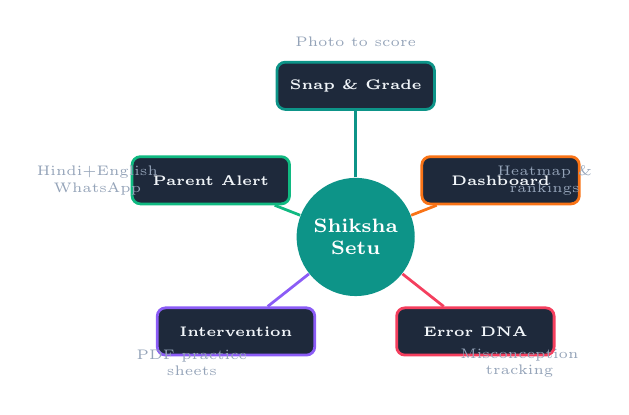
\begin{tikzpicture}[scale=0.80,
  hub/.style={circle, fill=teal, text=white, font=\bfseries\scriptsize,
              minimum size=1.5cm, align=center},
  spoke/.style={rounded corners=3pt, fill=card,
                line width=1pt, text=txt, font=\bfseries\tiny,
                minimum width=2.0cm, minimum height=0.60cm, align=center}]
  \node[hub] (c) at (0,0) {Shiksha\\Setu};
  \node[spoke,draw=teal]   (a) at ( 0,    2.4) {Snap \& Grade};
  \node[spoke,draw=orng]   (b) at ( 2.3,  0.9) {Dashboard};
  \node[spoke,draw=red]    (d) at ( 1.9, -1.5) {Error DNA};
  \node[spoke,draw=purple] (e) at (-1.9, -1.5) {Intervention};
  \node[spoke,draw=green]  (f) at (-2.3,  0.9) {Parent Alert};
  \draw[teal,  line width=1pt] (c)--(a);
  \draw[orng,  line width=1pt] (c)--(b);
  \draw[red,   line width=1pt] (c)--(d);
  \draw[purple,line width=1pt] (c)--(e);
  \draw[green, line width=1pt] (c)--(f);
  \node[text=txtsec,font=\tiny,align=center] at (0,3.1)     {Photo to score};
  \node[text=txtsec,font=\tiny,align=center] at (3.0,0.9)   {Heatmap \&\\rankings};
  \node[text=txtsec,font=\tiny,align=center] at (2.6,-2.0)  {Misconception\\tracking};
  \node[text=txtsec,font=\tiny,align=center] at (-2.6,-2.0) {PDF practice\\sheets};
  \node[text=txtsec,font=\tiny,align=center] at (-4.1,0.9)  {Hindi+English\\WhatsApp};
\end{tikzpicture}
\end{center}

\column{0.52\textwidth}
\vspace{4pt}
\sectionbox{teal}{1. Snap \& Grade (AI Batch Grading)}{Photo of handwritten worksheet to JSON score in under 5 seconds. Parallel batches of 5.}
\sectionbox{orng}{2. Class Intelligence Dashboard}{Heatmap, peer rankings, score distribution, misconceptions, at-risk alerts -- all updating live.}
\sectionbox{purple}{3. Error DNA + Intervention Plans}{Tracks recurring misconceptions per student across all tests. One-click PDF practice sheets.}
\sectionbox{green}{4. Bilingual Parent Loop}{AI-generated Hindi + English WhatsApp message with practice PDF links -- ready in one tap.}

\end{columns}
\end{frame}

% ── SLIDE 6 : KEY USER FLOW ─────────────────────────────────
\begin{frame}[t,shrink=5]{Key User Flow}{End-to-End Teacher Journey}
\begin{columns}[T]

\column{0.54\textwidth}
\vspace{4pt}
\colorbox{card}{\parbox{0.92\linewidth}{\centering\vspace{3pt}
  \includegraphics[width=0.96\linewidth,height=0.54\textheight,keepaspectratio]{figures/userflow.png}\\[2pt]
  \textcolor{orng}{\scriptsize\bfseries PLEASE PLEASE ZOOM TO READ}
\vspace{3pt}}}

\column{0.42\textwidth}
\vspace{4pt}
\textcolor{teal}{\small\textbf{Flow Highlights}}\\[6pt]
\textcolor{txt}{\scriptsize\textbf{1.}} \textcolor{txt}{\scriptsize Teacher uploads worksheet photos}\\[4pt]
\textcolor{txt}{\scriptsize\textbf{2.}} \textcolor{txt}{\scriptsize AI grades in parallel batches of 5}\\[4pt]
\textcolor{orng}{\scriptsize\textbf{3.}} \textcolor{txt}{\scriptsize Confidence $<$ 0.72 \textrightarrow{} \textbf{Review Queue}}\\[4pt]
\textcolor{green}{\scriptsize\textbf{4.}} \textcolor{txt}{\scriptsize Teacher approves in one click}\\[4pt]
\textcolor{purple}{\scriptsize\textbf{5.}} \textcolor{txt}{\scriptsize Dashboard \& Error DNA update live}\\[4pt]
\textcolor{red}{\scriptsize\textbf{6.}} \textcolor{txt}{\scriptsize Intervention plan + WhatsApp message}\\[8pt]

\statrow{orng}{$<$5 sec}{Per worksheet, end-to-end}
\statrow{teal}{8--12}{Worksheets per minute (batch-parallel)}

\end{columns}
\end{frame}

% ── SLIDE 7 : WHY AI IS NECESSARY ───────────────────────────
\begin{frame}[t,shrink=5]{Why AI is Necessary}{What Breaks Without It}
\begin{columns}[T]

\column{0.48\textwidth}
\vspace{4pt}
\colorbox{card}{\parbox{0.92\linewidth}{%
  \vspace{4pt}
  \textcolor{red}{\small\textbf{Without AI}}\\[5pt]
  \textcolor{red}{\scriptsize$\times$} \textcolor{txt}{\scriptsize \textbf{3+ hours} to grade 60 handwritten tests manually}\\[3pt]
  \textcolor{red}{\scriptsize$\times$} \textcolor{txt}{\scriptsize Teacher marks score -- \textbf{never knows} which concept failed}\\[3pt]
  \textcolor{red}{\scriptsize$\times$} \textcolor{txt}{\scriptsize Class-wide error patterns are \textbf{invisible}}\\[3pt]
  \textcolor{red}{\scriptsize$\times$} \textcolor{txt}{\scriptsize At-risk students \textbf{not identified} until exam failure}\\[3pt]
  \textcolor{red}{\scriptsize$\times$} \textcolor{txt}{\scriptsize No scalable Hindi/Marathi OCR for handwritten work}\\[3pt]
  \textcolor{red}{\scriptsize$\times$} \textcolor{txt}{\scriptsize Parent communication takes \textbf{hours} of teacher effort}\\[4pt]
}}

\column{0.48\textwidth}
\vspace{4pt}
\colorbox{card}{\parbox{0.92\linewidth}{%
  \vspace{4pt}
  \textcolor{green}{\small\textbf{With Shiksha Setu AI}}\\[5pt]
  \textcolor{green}{\scriptsize$\checkmark$} \textcolor{txt}{\scriptsize \textbf{$<$5 sec} per worksheet, 8--12 per minute in batches}\\[3pt]
  \textcolor{green}{\scriptsize$\checkmark$} \textcolor{txt}{\scriptsize \textbf{Concept-level} error mapping per question per student}\\[3pt]
  \textcolor{green}{\scriptsize$\checkmark$} \textcolor{txt}{\scriptsize Class-wide \textbf{heatmap} surfaces top 5 problem areas instantly}\\[3pt]
  \textcolor{green}{\scriptsize$\checkmark$} \textcolor{txt}{\scriptsize \textbf{Predictive risk tier} (high/medium/low) before next test}\\[3pt]
  \textcolor{green}{\scriptsize$\checkmark$} \textcolor{txt}{\scriptsize Handles \textbf{Hindi, Marathi, Devanagari, mixed-script} worksheets}\\[3pt]
  \textcolor{green}{\scriptsize$\checkmark$} \textcolor{txt}{\scriptsize \textbf{One-tap} bilingual parent message with PDF links}\\[4pt]
}}

\end{columns}
\vspace{6pt}
\colorbox{card}{\parbox{0.92\textwidth}{\centering\vspace{3pt}
  \textcolor{orng}{\small\textbf{Key Point:}}\;
  \textcolor{txt}{\small AI is not a convenience -- it is the \textit{only} path to per-concept
  diagnostics at 65-student-class scale without adding teacher workload.}
\vspace{3pt}}}
\end{frame}

% ── SLIDE 8 : AI METHODOLOGY ────────────────────────────────
\begin{frame}[t,shrink=5]{AI Methodology}{Model Choice \& Prompt Design}
\begin{columns}[T]

\column{0.50\textwidth}
\vspace{4pt}
\textcolor{teal}{\small\textbf{Model Stack}}\\[5pt]

\colorbox{card}{\parbox{0.92\linewidth}{%
  \vspace{3pt}
  \textcolor{teal}{\scriptsize\textbf{PRIMARY}}\; \textcolor{txt}{\scriptsize Claude Opus 4.1}\\
  \textcolor{txtsec}{\tiny claude-opus-4-1-20250805 \;|\; Anthropic Vision API \;|\; 4096 tokens}
\vspace{3pt}}}

\vspace{2pt}
\colorbox{card}{\parbox{0.92\linewidth}{\centering\vspace{1pt}
  \textcolor{orng}{\tiny $\downarrow$ On failure or rate-limit (3x exponential backoff)}
\vspace{1pt}}}
\vspace{2pt}

\colorbox{card}{\parbox{0.92\linewidth}{%
  \vspace{3pt}
  \textcolor{orng}{\scriptsize\textbf{FALLBACK}}\; \textcolor{txt}{\scriptsize Gemini 2.0 Flash}\\
  \textcolor{txtsec}{\tiny gemini-2.0-flash \;|\; Google GenAI \;|\; Same JSON contract}
\vspace{3pt}}}

\vspace{2pt}
\colorbox{card}{\parbox{0.92\linewidth}{\centering\vspace{1pt}
  \textcolor{red}{\tiny $\downarrow$ Both fail}
\vspace{1pt}}}
\vspace{2pt}

\colorbox{card}{\parbox{0.92\linewidth}{%
  \vspace{3pt}
  \textcolor{red}{\scriptsize\textbf{SAFETY NET}}\; \textcolor{txt}{\scriptsize Manual Review}\\
  \textcolor{txtsec}{\tiny Flagged for teacher -- never silently dropped from dashboard}
\vspace{3pt}}}

\column{0.46\textwidth}
\vspace{4pt}
\textcolor{purple}{\small\textbf{Prompt Engineering Choices}}\\[5pt]
\sectionbox{purple}{Tri-state grading decision}{\texttt{graded} / \texttt{needs\_teacher\_review} / \texttt{manual\_review}}
\sectionbox{teal}{Confidence per question}{0 to 1 float; threshold 0.72 triggers the review queue}
\sectionbox{orng}{Answer key injection}{Teacher's key overrides LLM -- becomes ground truth}
\sectionbox{green}{Multilingual support}{EN / HI / MR / Devanagari / mixed-script -- never rejected for language}

\vspace{2pt}
\colorbox{card}{\parbox{0.92\linewidth}{\centering\vspace{3pt}
  \textcolor{teal}{\textbf{0.72}}\; \textcolor{txtsec}{\scriptsize confidence threshold -- below this, teacher reviews before grade counts}
\vspace{3pt}}}

\end{columns}
\end{frame}

% ── SLIDE 9 : AI PIPELINE ───────────────────────────────────
\begin{frame}[t,shrink=5]{AI Grading Pipeline}{Inside the Grading Engine}
\begin{columns}[T]

\column{0.54\textwidth}
\vspace{4pt}
\colorbox{card}{\parbox{0.92\linewidth}{\centering\vspace{3pt}
  \includegraphics[width=0.96\linewidth,height=0.54\textheight,keepaspectratio]{figures/pipeline.png}\\[2pt]
  \textcolor{orng}{\scriptsize\bfseries PLEASE PLEASE ZOOM TO READ}
\vspace{3pt}}}

\column{0.42\textwidth}
\vspace{4pt}
\textcolor{orng}{\small\textbf{Safety Layers}}\\[5pt]
\sectionbox{teal}{Image validation}{Magic-byte check, MIME verify, 4 MB cap}
\sectionbox{teal}{JSON schema enforcement}{All fields normalised; missing fields get safe defaults}
\sectionbox{teal}{Confidence gating}{Low-confidence questions sent to teacher review queue}
\sectionbox{teal}{Score clamping}{Always 0--100, finite, rounded integer}
\sectionbox{teal}{Graceful degradation}{Any failure \textrightarrow{} Manual Review; nothing silently dropped}

\vspace{4pt}
\colorbox{card}{\parbox{0.92\linewidth}{\centering\vspace{3pt}
  \textcolor{teal}{\small\textbf{In-memory only}}\;
  \textcolor{txtsec}{\scriptsize Worksheet images are never persisted to the database}
\vspace{3pt}}}

\end{columns}
\end{frame}

% ── SLIDE 10 : HUMAN IN THE LOOP ────────────────────────────
\begin{frame}[t,shrink=5]{Human-in-the-Loop Safety}{AI Suggests, Teacher Decides}
\begin{columns}[T]

\column{0.50\textwidth}
\vspace{4pt}
\textcolor{purple}{\small\textbf{Review Queue Flow}}\\[5pt]
\colorbox{card}{\parbox{0.92\linewidth}{\centering\vspace{3pt}
  \includegraphics[width=0.96\linewidth,height=0.54\textheight,keepaspectratio]{figures/reviewqueue.png}\\[2pt]
  \textcolor{orng}{\scriptsize\bfseries PLEASE PLEASE ZOOM TO READ}
\vspace{3pt}}}

\column{0.46\textwidth}
\vspace{4pt}
\sectionbox{purple}{What lands in the Review Queue?}{Any worksheet where at least one question's confidence is below \textbf{0.72} -- readable but ambiguous.}
\sectionbox{green}{Approved grades}{Move into dashboard analytics and the student's permanent test timeline.}
\sectionbox{red}{Manual Review flags}{Unreadable, non-math, or corrupted images. Never silently affect the class average.}
\vspace{6pt}
\colorbox{card}{\parbox{0.92\linewidth}{%
  \vspace{3pt}
  \textcolor{txt}{\scriptsize\textbf{Design principle:}}\\
  \textcolor{txtsec}{\scriptsize A wrong AI grade that silently enters the dashboard is worse than no grade at all. The queue exists to prevent exactly that.}
\vspace{3pt}}}

\end{columns}
\end{frame}

% ── SLIDE 11 : AI EVALUATION PLAN ───────────────────────────
\begin{frame}[t,shrink=5]{AI Evaluation Plan}{How We Measure Performance}
\begin{columns}[T]

\column{0.56\textwidth}
\vspace{4pt}
\textcolor{teal}{\small\textbf{Evaluation Metrics \& Targets}}\\[5pt]
\renewcommand{\arraystretch}{1.5}
\colorbox{card}{\parbox{0.92\linewidth}{%
\vspace{3pt}
\begin{tabular}{@{\,}p{2.6cm}p{1.1cm}p{3.2cm}@{}}
  \textcolor{teallt}{\tiny\bfseries Metric} &
  \textcolor{orng}{\tiny\bfseries Target} &
  \textcolor{txtsec}{\tiny\bfseries Approach} \\
  \midrule
  \textcolor{txt}{\tiny Score MAE} &
  \textcolor{green}{\tiny\bfseries $<$8 pts} &
  \textcolor{txtsec}{\tiny Expert-graded gold set (n=120)} \\
  \textcolor{txt}{\tiny Manual review rate} &
  \textcolor{green}{\tiny\bfseries $<$5\%} &
  \textcolor{txtsec}{\tiny Clear + degraded image mix} \\
  \textcolor{txt}{\tiny Concept F1 score} &
  \textcolor{green}{\tiny\bfseries $>$0.80} &
  \textcolor{txtsec}{\tiny Concept-tagged question set} \\
  \textcolor{txt}{\tiny Confidence calibration} &
  \textcolor{green}{\tiny\bfseries ECE $<$0.10} &
  \textcolor{txtsec}{\tiny Binned accuracy vs confidence} \\
  \textcolor{txt}{\tiny Throughput} &
  \textcolor{green}{\tiny\bfseries 8--12/min} &
  \textcolor{txtsec}{\tiny Batch-parallel load test} \\
  \textcolor{txt}{\tiny Teacher SUS} &
  \textcolor{green}{\tiny\bfseries $\geq$75} &
  \textcolor{txtsec}{\tiny 5-teacher usability study} \\
\end{tabular}
\vspace{3pt}}}

\vspace{5pt}
\colorbox{card}{\parbox{0.92\linewidth}{%
  \vspace{3pt}
  \textcolor{orng}{\scriptsize\textbf{Test Set Design -- n = 120 diverse worksheets:}}\\
  \textcolor{txtsec}{\tiny 9 math concepts $\times$ 3 difficulty levels $\times$ 3 script types (EN/HI/mixed) $\times$ 2 image quality tiers (clean/degraded). Expert teacher graded as gold standard.}
\vspace{3pt}}}

\column{0.70\textwidth}
\vspace{4pt}
\textcolor{purple}{\small\textbf{Test Set Rationale}}\\[2pt]
\sectionbox{purple}{Concept diversity}{9 topics: Algebra, Trig, Calculus, Probability, Geometry}
\sectionbox{orng}{Script diversity}{English, Hindi (Devanagari), mixed-language worksheets}
\sectionbox{teal}{Image quality range}{Clean scans AND blurry phone photos to stress-test OCR}
\sectionbox{red}{Edge cases}{Blank pages, non-math uploads, partial submissions}
\sectionbox{green}{Double-blind scoring}{Two teachers grade independently; third resolves disagreements}

\end{columns}
\end{frame}

% ── SLIDE 12 : SYSTEM ARCHITECTURE ─────────────────────────
\begin{frame}[t]{System Architecture}{High-Level Technical Design}

\begin{center}
  \includegraphics[width=1.20\textwidth,height=0.74\textheight,keepaspectratio]{figures/architecture.png}\\[2pt]
  \textcolor{orng}{\scriptsize\bfseries PLEASE PLEASE ZOOM TO READ}
\end{center}
\end{frame}

\begin{frame}[t,shrink=5]{System Architecture}{High-Level Technical Design}
\begin{columns}[T]

\column{0.52\textwidth}
\vspace{-4pt}
\textcolor{teal}{\small\textbf{Layer Breakdown}}\\[5pt]
\renewcommand{\arraystretch}{1.4}
\colorbox{card}{\parbox{0.92\linewidth}{%
\vspace{3pt}
\begin{tabular}{@{\,}p{1.5cm}p{4.2cm}@{}}
  \textcolor{teallt}{\scriptsize\bfseries Frontend} &
    \textcolor{txtsec}{\tiny React 19 + Vite, PWA, Service Worker, i18n (EN/HI/MR)}\\
  \textcolor{orng}{\scriptsize\bfseries API Layer} &
    \textcolor{txtsec}{\tiny Express 5 on Vercel Serverless, session-scoped, Multer in-memory}\\
  \textcolor{purple}{\scriptsize\bfseries AI Layer} &
    \textcolor{txtsec}{\tiny Claude Opus 4.1 (primary) \textrightarrow{} Gemini 2.0 Flash (fallback)}\\
  \textcolor{green}{\scriptsize\bfseries Database} &
    \textcolor{txtsec}{\tiny MongoDB Atlas -- Student, Submission, GradingSession, GradingRun}\\
  \textcolor{yellow}{\scriptsize\bfseries CDN} &
    \textcolor{txtsec}{\tiny Vercel Edge -- React SPA + 9 practice PDFs served statically}\\
\end{tabular}
\vspace{3pt}}}

\column{0.44\textwidth}
\vspace{-4pt}
\textcolor{orng}{\small\textbf{Key Design Decisions}}\\[4pt]
\sectionbox{teal}{Images in-memory only}{Worksheet buffers never persisted to the database}
\sectionbox{teal}{Session-scoped isolation}{Each grading run is UUID-isolated; no cross-session leakage}
\sectionbox{teal}{Offline upload queue}{Frontend stores worksheets locally; auto-syncs on reconnect}

\end{columns}
\end{frame}

% ── SLIDE 13 : REAL-WORLD READINESS ─────────────────────────
\begin{frame}[t,shrink=5]{Real-World Readiness}{Built for India's Classrooms}
\begin{columns}[T]
\vspace{-2pt}
\column{0.48\textwidth}

\textcolor{teal}{\small\textbf{Low Connectivity}}\\
\sectionbox{teal}{PWA + Service Worker}{App shell cached on install -- loads on 2G networks}
\sectionbox{teal}{Offline upload queue}{Worksheets saved locally, auto-sync when signal returns}
\sectionbox{teal}{Data cost display}{Live rupee-per-worksheet estimate for metered connections}

\vspace{2pt}
\textcolor{purple}{\small\textbf{Entry-Level Devices}}\\[1pt]
\sectionbox{purple}{4 MB image cap}{Works with basic Android camera quality}
\sectionbox{purple}{Cache-first strategy}{Static assets served instantly from service worker cache}
\sectionbox{purple}{No native app required}{Runs in mobile Chrome -- zero install friction}

\column{0.48\textwidth}
\textcolor{orng}{\small\textbf{Regional Languages}}\\[4pt]
\sectionbox{orng}{Full UI in 3 languages}{English, Hindi, Marathi -- persisted to localStorage}
\sectionbox{orng}{Multilingual worksheet grading}{EN/HI/MR/Devanagari -- never rejected for language}
\sectionbox{orng}{Bilingual parent messages}{AI generates Hindi + English WhatsApp text with PDF links}

\vspace{2pt}
\textcolor{green}{\small\textbf{Cost Reality Check}}\\[4pt]
\colorbox{card}{\parbox{0.92\linewidth}{%
\vspace{3pt}
\renewcommand{\arraystretch}{1.3}
\begin{tabular}{@{\,}p{4.5cm}r@{\,}}
  \textcolor{txtsec}{\scriptsize Claude API (750 sheets/month)} & \textcolor{green}{\scriptsize\bfseries Rs.\ 525}\\
  \textcolor{txtsec}{\scriptsize Vercel + MongoDB infra}        & \textcolor{green}{\scriptsize\bfseries Rs.\ 260}\\
  \textcolor{txt}{\scriptsize\bfseries Total / classroom / month} & \textcolor{orng}{\scriptsize\bfseries Rs.\ 785}\\
  \textcolor{txtsec}{\scriptsize Per student (50 students)}     & \textcolor{teal}{\scriptsize\bfseries Rs.\ 1.05}\\
\end{tabular}
\vspace{3pt}}}

\end{columns}
\end{frame}

% ============================================================
\end{document}
% ============================================================
